\documentclass[activite]{thedocument}
\startdatakeys
\source{}
\cycle{}
\competencesDuSocle{}
\connaissancesRequises{}
\competencesTravaillees{}
\enddatakeys
\begin{document}
    \noindent Le professeur demande à ses élèves : \guillemets{Le triangle suivant est-il constructible~?}
    \vskip15pt\noindent
    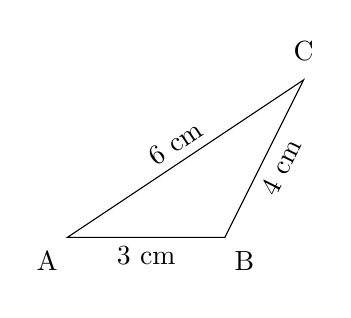
\begin{tikzpicture}
        \coordinate(A)at(0,0);
        \coordinate(B)at(2,0);
        \coordinate(C)at(3,2);
        \draw node[below left]at(A){\strut A};
        \draw node[below right]at(B){\strut B};
        \draw node[above]at(C){\strut C};
        \path(A)--(B)node[midway, below, sloped]{3 cm};
        \path(B)--(C)node[midway, below, sloped]{4 cm};
        \path(A)--(C)node[midway, above, sloped]{6 cm};
        \draw(A)--(B)--(C)--cycle;
    \end{tikzpicture}\hskip20pt\vskip10pt\noindent
    Irène dit : \guillemets{J'ai répondu en vérifiant les trois inégalités tiangulaires.}
    \vskip10pt\noindent
    Sophie répond : \guillemets{Il suffit de vérifier une seule inégalité pour trouver la réponse !}
    \vskip30pt\noindent Comment Sophie a-t-elle fait~?
    \dotedline\dotedline\dotedline\vskip10pt\noindent
    Conclusion :\dotedline\dotedline
\end{document}